%Declaramos la clase de documento
\documentclass[12pt, letterpaper]{article}

%Paquetes de idioma y codificación de caracteres
\usepackage[utf8]{inputenc}
\usepackage[spanish]{babel}

%Otros paquetes
\usepackage{graphicx}

%Dimensiones del Documento
\usepackage[left=2cm,right=2cm,top=2cm,bottom=2cm]{geometry}
\usepackage{graphicx}%para las figuras
\usepackage{float}%para usar [H]
\usepackage{amsmath}
\usepackage{enumerate}%para los enumerados
\usepackage{hyperref}
\renewcommand{\labelitemi}{$-$}
\renewcommand{\labelitemi}{$\cdot$}

%Datos para el titulo de nuestro documento
   %\title{Informe de Laboratorio N°07 - Base de Datos II}
   %\author{Gabriela Atahuachi Rivera}
   %\date{\today}

\begin{document}

%Imprimimos la pagina de titulo
\title{Caratula}

\begin{titlepage}
	\begin{center}
		\large{UNIVERSIDAD PRIVADA DE TACNA}\\

		\vspace*{-0.025in}
			\begin{figure}[htb]
				\begin{center}
					
\includegraphics[width=8cm]{./Imagenes/LogoUpt}
				\end{center}
			\end{figure}

		\vspace*{0.15in}
		INGENIERIA DE SISTEMAS  \\

		\vspace*{0.5in}
			\begin{large}
			TITULO:\\
			\end{large}

		\vspace*{0.1in}
			\begin{large}
				\textbf{Informe de Laboratorio 7} \\
				\textbf{Instalación de una Instancia de Microsoft SQL Server} \\
			\end{large}

		\vspace*{0.3in}
			\begin{large}
				\textbf{CURSO:} \\
			\end{large}

		\vspace*{0.1in}
			\begin{large}
				Base De Datos II \\
			\end{large}

		\vspace*{0.3in}
			\begin{large}
				\textbf{DOCENTE:} \\
			\end{large}

		\vspace*{0.1in}
			\begin{large}
				Ing. Patrick Cuadros Quiroga \\
			\end{large}

		\vspace*{0.2in}
			\vspace*{0.1in}
				\begin{large}
					Integrantes: \\
					\begin{flushleft}
						Atahuachi Rivera, Gabriela Atahuachi	\hfill	(2016055341) \\
					\end{flushleft}
				\end{large}
	\end{center}
\end{titlepage}

\tableofcontents %para el índice
	\thispagestyle{empty} %para el índice sin numero
		\newpage
			\setcounter{page}{1}%reiniciar contador de paginas despues del indice
				\section{Información General}

	\begin{itemize}
		\subsection{Objetivos:}
			\item Descarga e Instalación del Docker Desktop
			 \item Poder Configurar Correctamente el Docker Desktop en PowerShell
			 \item Poder Instalar Correctamente las Consultas Requeridas
		\subsection{Recursos Utilizados:}
			\item Al menos 4 GB de RAM.
			\item Windows 10 64-bit: Pro, Enterprise o Education
			\item Docker Desktop
			\item Microsoft SQL Server Management Studio (Última Versión)
			\item Necesariamente Internet para la Descarga
		\subsection{Conocimientos:}
			\item Conocimientos Básicos de Administracion de Base de Datos Microsoft SQL Server.
			\item Conocimientos Basicos de SQL.
	\end{itemize}
				\section{Procedimientos.}

	\begin{itemize}
		\subsection{Descarga del Software.}
			\item Ingresamos a Nuestro Buscador de Internet Google Chrome  o cualquier otro.
				\begin{figure}[htb]
					\begin{center}
						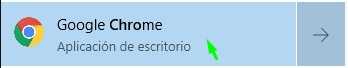
\includegraphics[width=8cm]{./Imagenes/BuscarAppGoogle}
					\end{center}
				\end{figure}
			\item Luego Copiamos y Pegamos el Siguiente Link.
				\begin{center}
					\url{https://hub.docker.com/search/?type=edition&offering=community}
				\end{center}
			\item Luego aparecerá esta pestaña, por lo que debemos primeramente tener una cuenta en Docker.
				\begin{figure}[htb]
					\begin{center}
						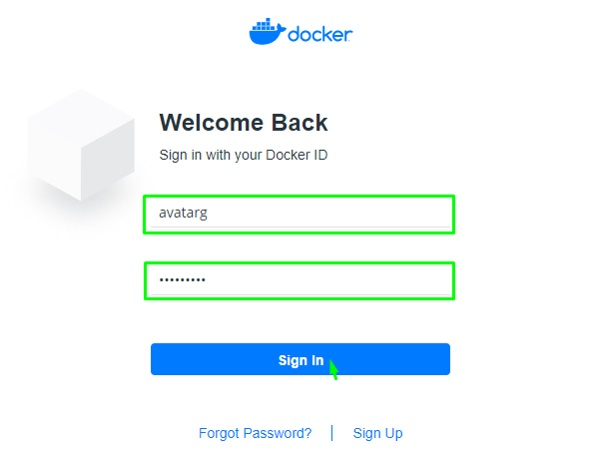
\includegraphics[width=9cm]{./Imagenes/Loguearse}
					\end{center}
				\end{figure}			
			\item Luego aparecerán varias aplicaciones para descargar del Docker, nos movemos hacia abajo con el mouse.
				\begin{figure}[htb]
					\begin{center}
						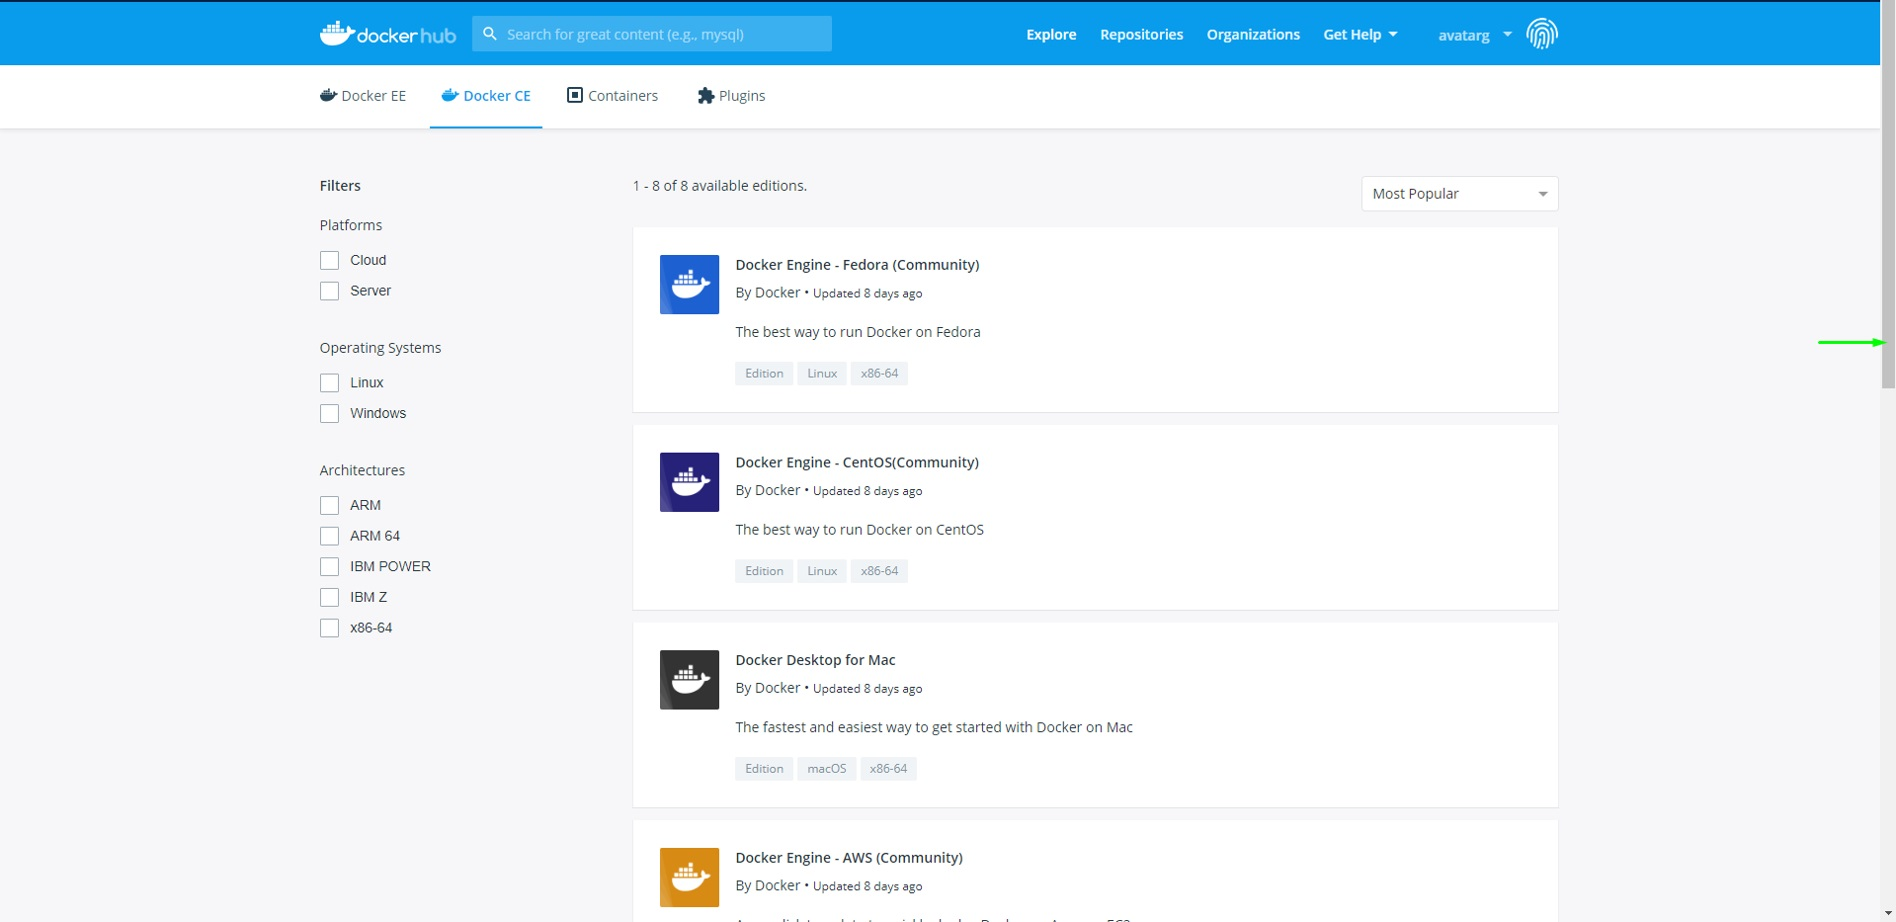
\includegraphics[width=19cm]{./Imagenes/VariasApps}
					\end{center}
				\end{figure}
				\vspace{7cm}
			\item Una vez hecho esto, nos llevará a una ventana para obtener el ejecutable del Docker.
				\begin{figure}[htb]
					\begin{center}
						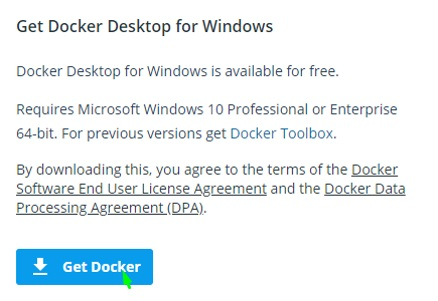
\includegraphics[width=10cm]{./Imagenes/ObtenerApp2}
					\end{center}
				\end{figure}
			\item Seleccionamos esta pestaña.
				\begin{figure}[htb]
					\begin{center}
						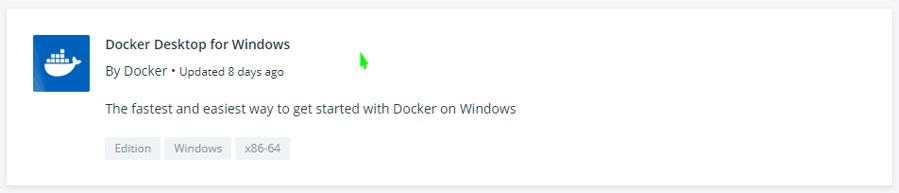
\includegraphics[width=12cm]{./Imagenes/SeleccionarApp}
					\end{center}
				\end{figure}
				\vspace{5cm}
			\item Y empezará la descarga del ejecutable de Docker Desktop. Solo esperar a que termine la descarga, esto puede tomar varios minutos dependiendo de la velocidad del internet.
				\begin{figure}[htb]
					\begin{center}
						
\includegraphics[width=8cm]{./Imagenes/DescargarEjecutableApp}
					\end{center}
				\end{figure}
		\subsection{Instalación del Docker Desktop}
			\item Una vez ya terminada la descarga del ejecutable, la seleccionamos para empezar la instalación.
				\begin{figure}[htb]
					\begin{center}
						
\includegraphics[width=8cm]{./Imagenes/EjecutarEjecutableApp}
					\end{center}
				\end{figure}
			\item Y aparecerá esta ventana indicando la inicialización de la instalación. Esperamos unos segundos hasta que aparezca otra ventana.
				\begin{figure}[htb]
					\begin{center}
						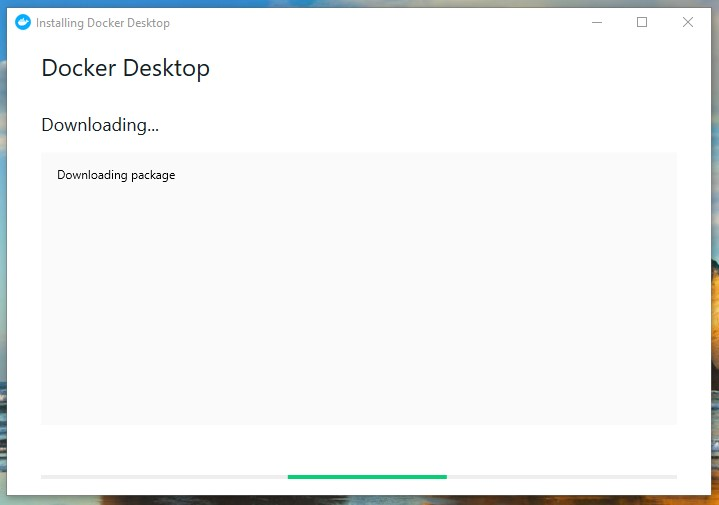
\includegraphics[width=11cm]{./Imagenes/Instalacion01}
					\end{center}
				\end{figure}
				\vspace{10cm}
			\item Luego nos pedirá confirmación de si Aceptamos Añadir un Acceso Directo al Escritorio de nuestra Maquina.
				\begin{figure}[htb]
					\begin{center}
						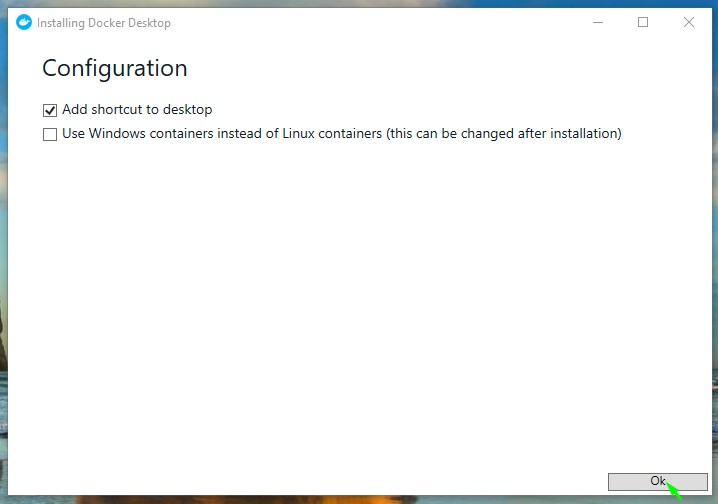
\includegraphics[width=11cm]{./Imagenes/Instalacion02}
					\end{center}
				\end{figure}
			\item Comenzará la instalación de cada paquete. Solo esperar hasta que termine.
				\begin{figure}[htb]
					\begin{center}
						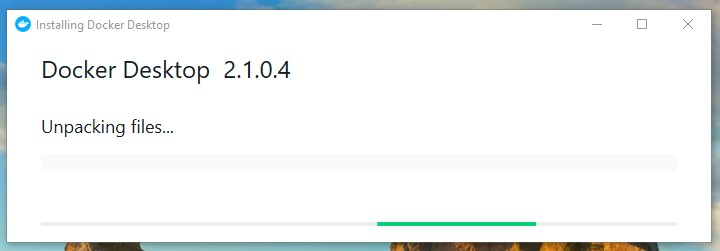
\includegraphics[width=11cm]{./Imagenes/Instalacion03}
					\end{center}
				\end{figure}
				\vspace{10cm}
			\item Durante la instalación de Docker, ya aparecerá el icono del Software en el escritorio, tal como se muestra en la siguiente imagen.
				\begin{figure}[htb]
					\begin{center}
						
\includegraphics[width=2cm]{./Imagenes/NuevoIcono}
					\end{center}
				\end{figure}
				%\vspace{5cm}
			\item Una vez terminada la instalación de Docker, seleccionamos el botón como aparece en la imagen y se reiniciará el equipo para actualizar y guardar las configuraciones hechas.
				\begin{figure}[htb]
					\begin{center}
						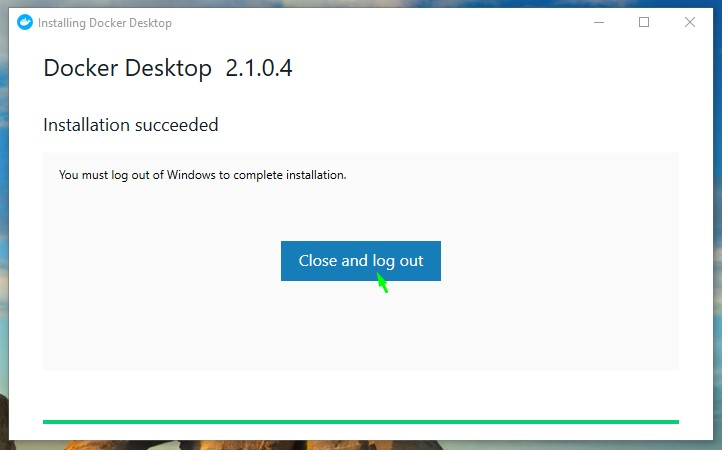
\includegraphics[width=11cm]{./Imagenes/Instalacion05}
					\end{center}
				\end{figure}
				%\vspace{3cm}
		\subsection{Creación de Carpetas a Usar}
			\item Después de reiniciar la máquina, creamos dos carpetas en la unidad que desee, en mi caso lo crearé en el disco D.
				\begin{figure}[htb]
					\begin{center}
						
\includegraphics[width=3cm]{./Imagenes/CarpetasCreadas}
					\end{center}
				\end{figure}
				\vspace{3cm}
		\subsection{Configuración por PowerShell}
			\subsubsection{Parte 1. Aplicación en Ejecución}
				\item Luego aparecerá por defecto una notificación del Sistema Operativo.
					\begin{figure}[htb]
						\begin{center}
							
\includegraphics[width=8cm]{./Imagenes/IniciacionDocker}
						\end{center}
					\end{figure}
				\item Y se agregará un icono en la barra de tareas en la parte inferior derecho.
					\begin{figure}[htb]
						\begin{center}
							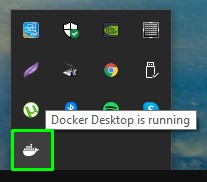
\includegraphics[width=6cm]{./Imagenes/IconoDeIniciacion}
						\end{center}
					\end{figure}
			\subsubsection{Parte 2. Buscar PoweShell}
				\item Ahora buscamos el programa Windows PowerShell.
					\begin{figure}[htb]
						\begin{center}
							
\includegraphics[width=8cm]{./Imagenes/BuscarPowerShell}
						\end{center}
					\end{figure}
					\vspace{8cm}
				\item Luego lo ejecutamos como administrador para que no genere problemas luego.
					\begin{figure}[htb]
						\begin{center}
							
\includegraphics[width=6cm]{./Imagenes/EjecutarComoAdministrador}
						\end{center}
					\end{figure}
				\item Se mostrará una ventana como la que se ve en la imagen.
					\begin{figure}[htb]
						\begin{center}
							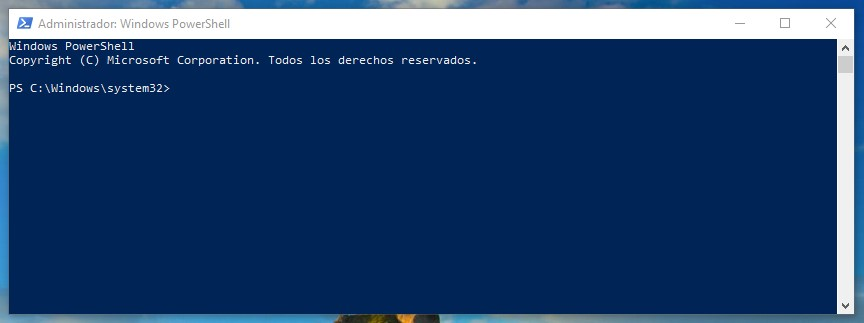
\includegraphics[width=16cm]{./Imagenes/InicioPowerShell}
						\end{center}
					\end{figure}
			\subsubsection{Parte 3. Verificar la Version de Docker Desktop}
				\item Luego, digitamos lo siguiente para Verificar la Versión del Docker que hemos instalado.
					\begin{center}
						\textbf{docker version} \\
					\end{center}
				\item El resultado sería como se muestra en la siguiente imagen.
					\begin{figure}[htb]
						\begin{center}
							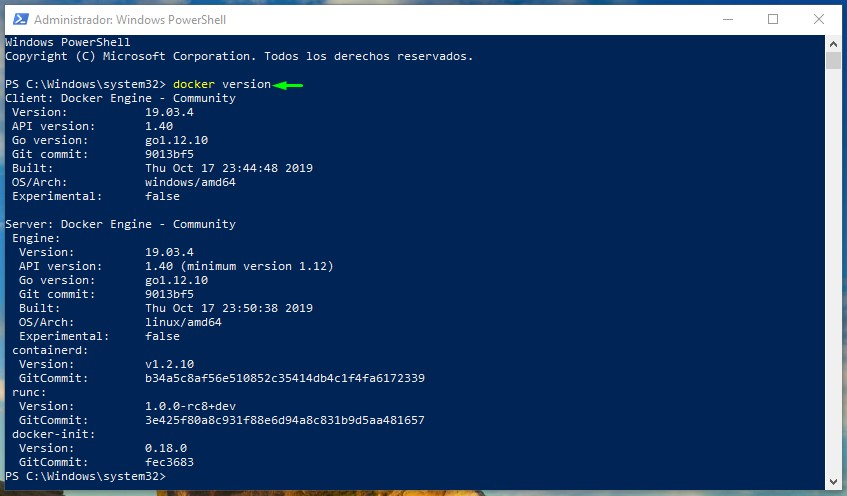
\includegraphics[width=16cm]{./Imagenes/VersionDocker}
						\end{center}
					\end{figure}
					\vspace{10cm}
			\subsubsection{Parte 4. Creación de un Contenedor con Microsoft SQL Server para Linux.}
				\item Digitarremos el siguiente comando.
					\begin{center}
						\textbf{docker search mssql}
					\end{center}
				\item El resultado sería similar a como se ve en la imagen.
					\begin{figure}[htb]
						\begin{center}
							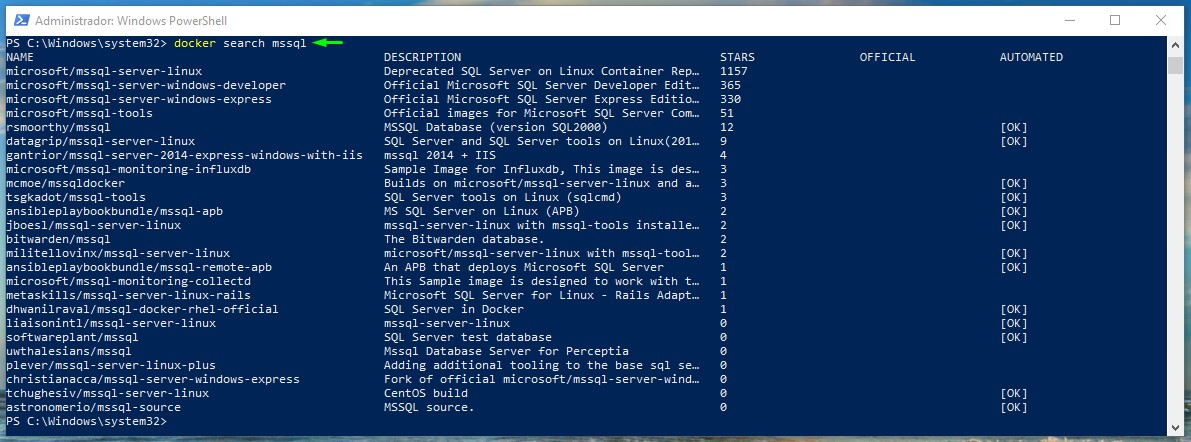
\includegraphics[width=16cm]{./Imagenes/Comando02}
						\end{center}
					\end{figure}
				\item{Procedemos a digitar el siguiente comando.}
					\begin{center}
						\textbf{docker pull microsoft/mssql-server-linux} \\
					\end{center}
				\item Y empezará la descargara de imagen de contenedor de Microsoft SQL Server en un servidor Linux.
					\begin{figure}[htb]
						\begin{center}
							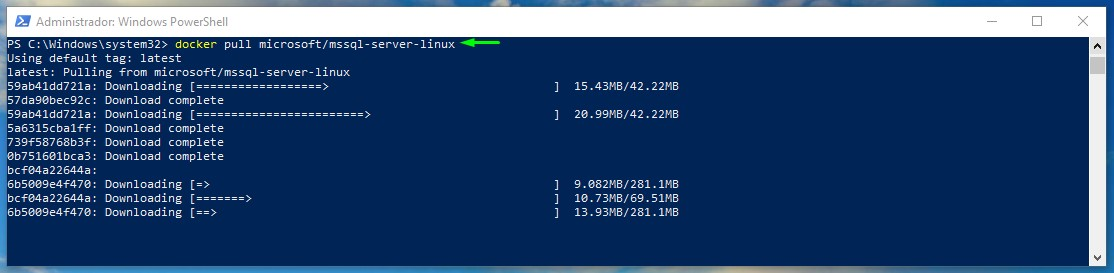
\includegraphics[width=16cm]{./Imagenes/Comando03}
						\end{center}
					\end{figure}
				\item Luego digitamos el siguiente comando.
					\begin{center}
						\textbf{docker images} \\
					\end{center}
				\item Lo cual se verificará la imagen.
					\begin{figure}[htb]
						\begin{center}
							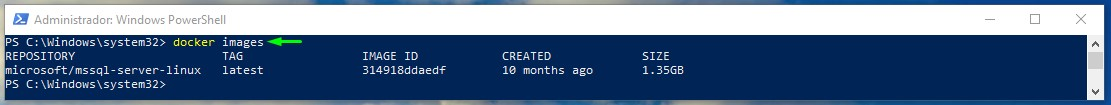
\includegraphics[width=16cm]{./Imagenes/Comando04}
						\end{center}
					\end{figure}
				\item Seguidamente ejecutamos el comando, como se muestra en la imagen y como respuesta se vizualizará un ID que corresponde al contenedor, como se muestra en la imagen.
					\begin{figure}[htb]
						\begin{center}
							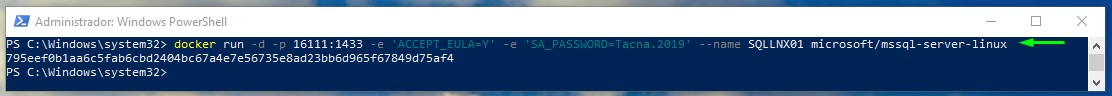
\includegraphics[width=16cm]{./Imagenes/Comando05}
						\end{center}
					\end{figure}
				\item Ejecutamos el siguiente comando.
					\begin{center}
						\textbf{docker ps} \\
					\end{center}
				\item Para verificar que el contenedor se este ejecutando correctamente.
					\begin{figure}[htb]
						\begin{center}
							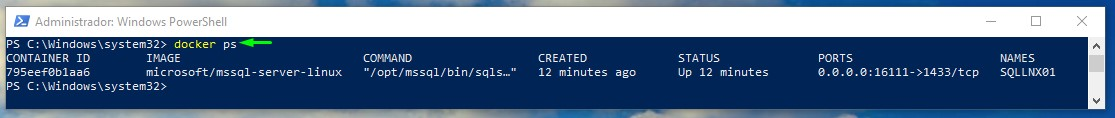
\includegraphics[width=16cm]{./Imagenes/Comando06}
						\end{center}
					\end{figure}
					\vspace{6cm}
				\item Esperamos unos segundos.
			\subsection{Consulta en SQL Server}
				\item Buscamos la Aplicación Microsoft SQL Server.
					\begin{figure}[htb]
						\begin{center}
							
\includegraphics[width=8cm]{./Imagenes/BuscarSQL}
						\end{center}
					\end{figure}
				\item Primeramente aparecerá esta pestaña y comenzara a cargar el programa.
					\begin{figure}[htb]
						\begin{center}
							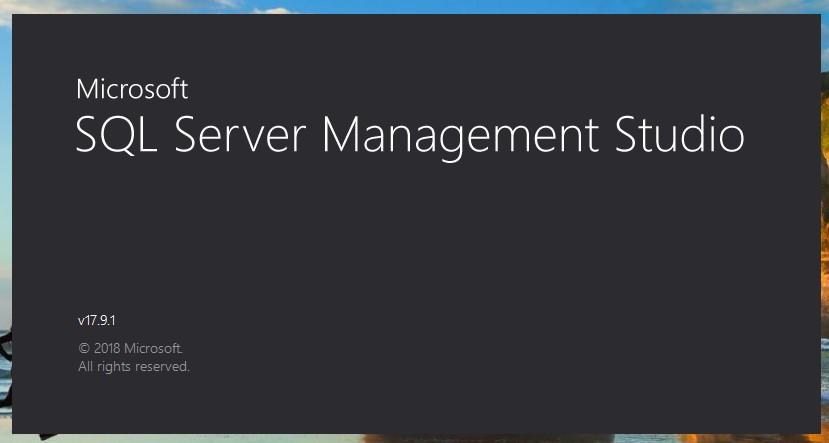
\includegraphics[width=12cm]{./Imagenes/InicioSql}
						\end{center}
					\end{figure}
				\item Se puede observar que por defecto se autentica con el nombre de tu maquina, como en mi caso, HARUKAATAHUACHI
					\begin{figure}[htb]
						\begin{center}
							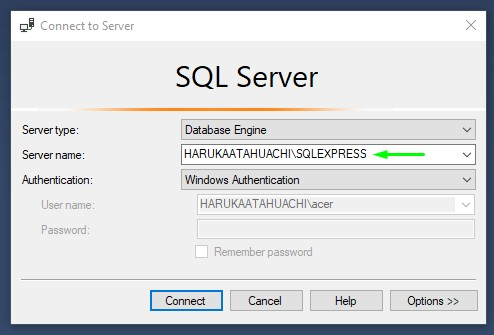
\includegraphics[width=12cm]{./Imagenes/ConectarseSql01}
						\end{center}
					\end{figure}
					\vspace{7cm}
				\item Ingresamos estos datos por los que se muestra en la imagen para conectarnos a Microsoft SQL Server Management Studio.
					\begin{figure}[htb]
						\begin{center}
							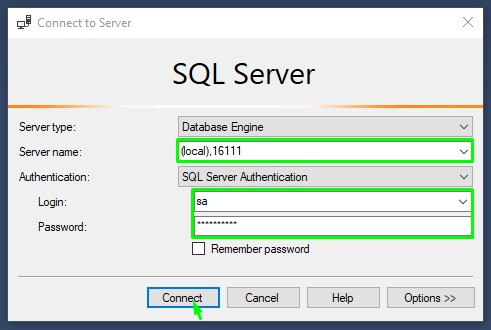
\includegraphics[width=12cm]{./Imagenes/ConectarseSql02}
						\end{center}
					\end{figure}
				\item Y ya hemos ingresado a la base de datos por medio del servidor, como se muestra en la imagen.
					\begin{figure}[htb]
						\begin{center}
							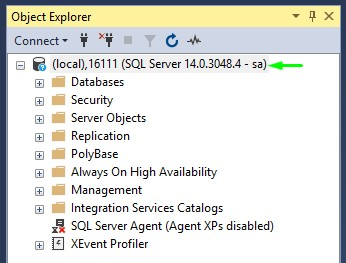
\includegraphics[width=10cm]{./Imagenes/ServidorLocal}
						\end{center}
					\end{figure}
					\vspace{5cm}
				\item Seleccionamos en el boton que se muestra en la imagen para agregar una consulta.
					\begin{figure}[htb]
						\begin{center}
							
\includegraphics[width=3cm]{./Imagenes/NuevaConsulta}
						\end{center}
					\end{figure}
				\item Digitaremos lo siguiente.
					\begin{center}
						\textbf{SELECT @@VERSION} \\
					\end{center}
				\item Seleccionamos y ejecutamos la consulta.
					\begin{figure}[htb]
						\begin{center}
							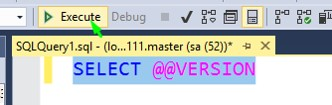
\includegraphics[width=12cm]{./Imagenes/EjecutarConsulta01}
						\end{center}
					\end{figure}
				\item Como resultado aparecerá esto.
					\begin{figure}[htb]
						\begin{center}
							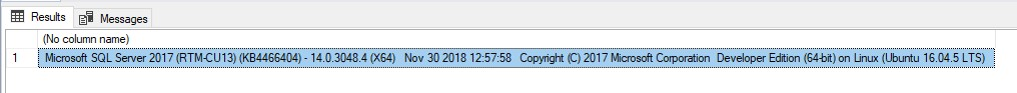
\includegraphics[width=19cm]{./Imagenes/ResultadoConsulta01}
						\end{center}
					\end{figure}
					\vspace{4cm}
			\subsection{De nuevo en PowerShell - Eliminar contenedor creado}
				\item Ahora cerramos la aplicación Microsoft SQL Server Management Studio.
					\begin{figure}[htb]
						\begin{center}
							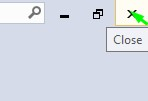
\includegraphics[width=8cm]{./Imagenes/CerrarSql}
						\end{center}
					\end{figure}
				\item De nuevo en PowerShell, digitamos el siguiente codigo.
					\begin{center}
						\textbf{docker rm -f SQLLNX01} \\
					\end{center}
				\item Lo ejecutamos y tendremos como resultado.
					\begin{figure}[htb]
						\begin{center}
							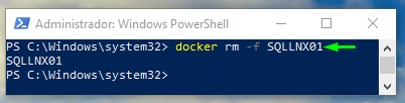
\includegraphics[width=8cm]{./Imagenes/Comando07}
						\end{center}
					\end{figure}
				\item Luego digitamos este comando nuevamente.
					\begin{center}
						\textbf{docker ps} \\
					\end{center}
				\item Lo ejecutamos y tendremos como resultado la elimnacion del contenedor creado.
					\begin{figure}[htb]
						\begin{center}
							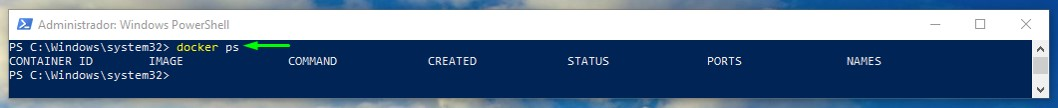
\includegraphics[width=19cm]{./Imagenes/Comando08}
						\end{center}
					\end{figure}
					\vspace{5cm}
			\subsection{Adicionando Persistencia.}
				\subsubsection{Parte 1. Primeramente en PowerShell}
					\item Digitaremos el siguiente comando, como se muestra en la imagen y como respuesta se vizualizará un ID que corresponde al contenedor.
						\begin{figure}[htb]
							\begin{center}
								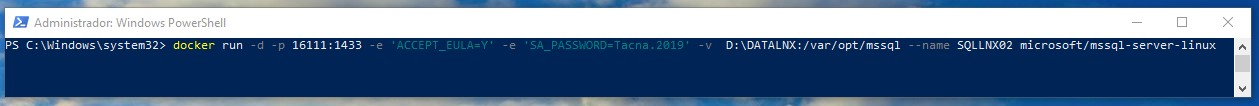
\includegraphics[width=19cm]{./Imagenes/Comando09}
							\end{center}
						\end{figure}
					\item Luego aparecerá esta pestaña para verificar los datos de la máquina.
						\begin{figure}[htb]
							\begin{center}
								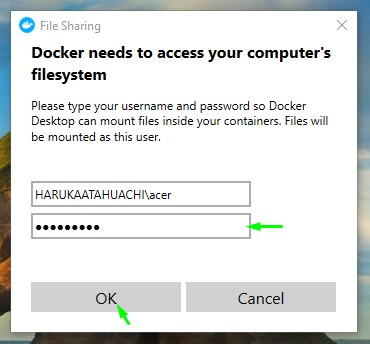
\includegraphics[width=10cm]{./Imagenes/Access02}
							\end{center}
						\end{figure}
					\item Y finalmente aparecerá la ID que corresponde al contenedor.
						\begin{figure}[htb]
							\begin{center}
								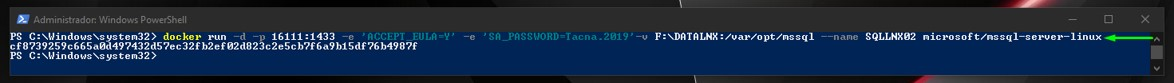
\includegraphics[width=19cm]{./Imagenes/Comando010}
							\end{center}
						\end{figure}
						\vspace{3cm}
					\item Ejecutamos de nuevo este comando 
						\begin{center}
							\textbf{docker ps} \\
						\end{center}
					\item Y obtendremos como resultado lo que se muestra en la imagen.
						\begin{figure}[htb]
							\begin{center}
								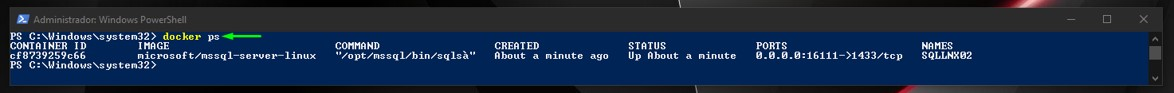
\includegraphics[width=19cm]{./Imagenes/Comando011}
							\end{center}
						\end{figure}
				\subsubsection{Parte 2. Seguidamente en Microsoft SQL Server Management}
					\item Buscamos de nuevo el programa Microsoft SQL Server.
						\begin{figure}[htb]
							\begin{center}
								
\includegraphics[width=8cm]{./Imagenes/BuscarSQL}
							\end{center}
						\end{figure}
					\item Se puede observar que por defecto se autentica con el nombre de tu maquina, como en mi caso, HARUKAATAHUACHI
						\begin{figure}[htb]
							\begin{center}
								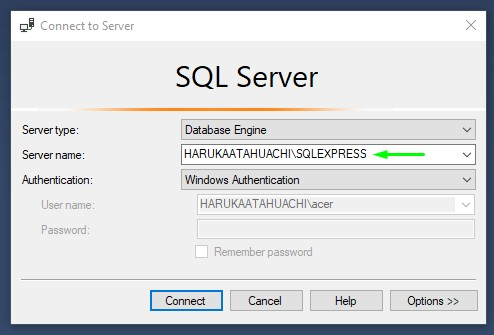
\includegraphics[width=12cm]{./Imagenes/ConectarseSql01}
							\end{center}
						\end{figure}
						\vspace{9cm}
					\item Volvemos a ingresar estos datos que se muestra en la imagen para conectarnos a Microsoft SQL Server Management Studio.
						 \begin{figure}[htb]
							\begin{center}
								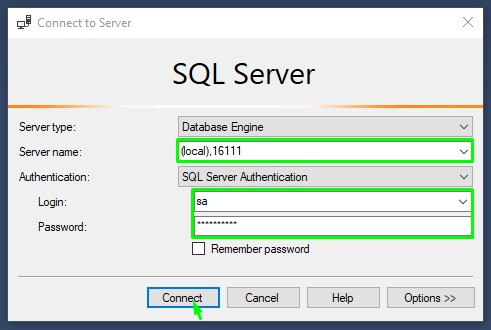
\includegraphics[width=12cm]{./Imagenes/ConectarseSql02}
							\end{center}
						\end{figure}
					\item Generamos una base de datos de prueba en la Aplicación Microsoft SQL Server Management Studio, según la siguiente imagen.
						\begin{figure}[htb]
							\begin{center}
								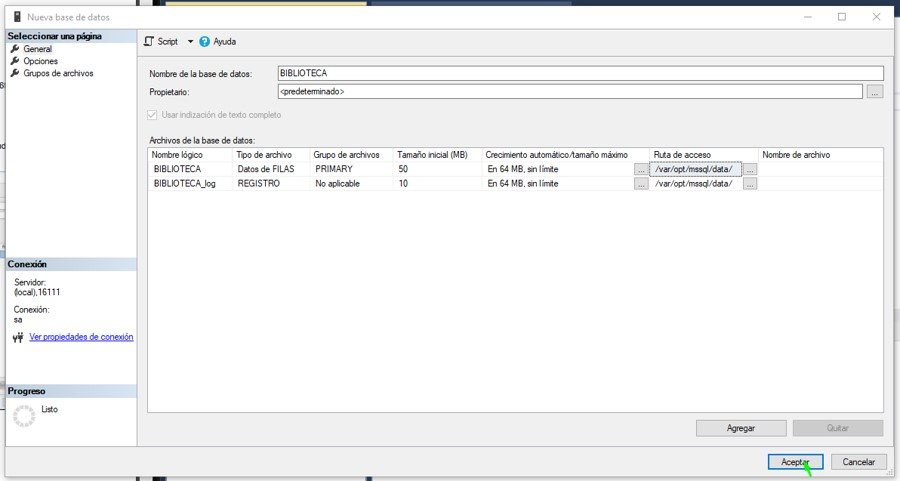
\includegraphics[width=18cm]{./Imagenes/GenerarDataBase}
							\end{center}
						\end{figure}
						\vspace{4cm}
					\item O sino mediante el siguiete script a continuación.
						\begin{figure}[htb]
							\begin{center}
								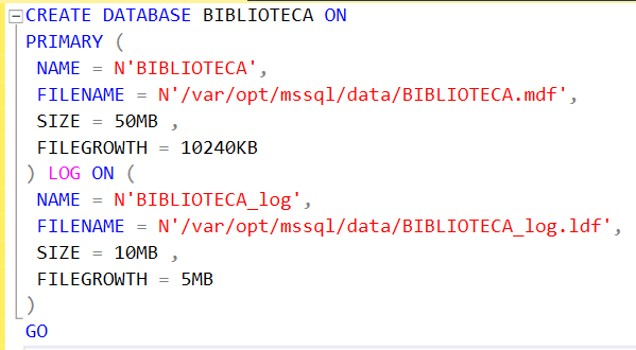
\includegraphics[width=16cm]{./Imagenes/CrearDataBase}
							\end{center}
						\end{figure}
						\vspace{12cm}
					\item Luego verificamos el contenido de la carpeta DATALNX.
						\begin{figure}[htb]
							\begin{center}
								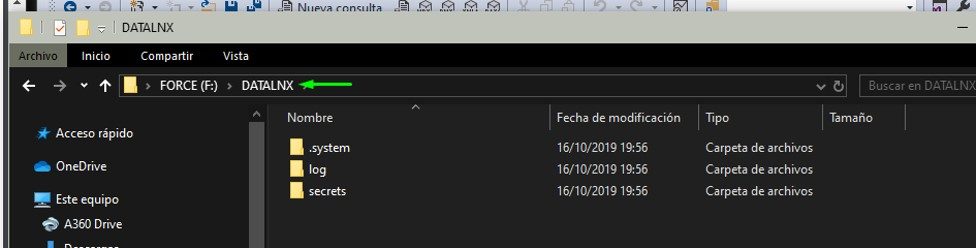
\includegraphics[width=16cm]{./Imagenes/VerificarDATALNX}
							\end{center}
						\end{figure}
				\subsubsection{Parte 3. Nuevamente en PowerShell}
					\item Ejecutamos el siguiente comando.
						\begin{center}
							\textbf{docker rm -f SQLLNX02} \\
						\end{center}
					\item Y el resultado será como se muestra en la siguiente imagen.
						\begin{figure}[htb]						
							\begin{center}
								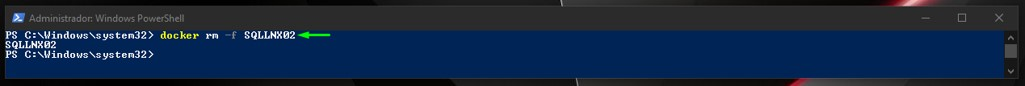
\includegraphics[width=19cm]{./Imagenes/Comando012}
							\end{center}
						\end{figure}
					\item Finalmente ejecutamos el siguiente codigo para verificar la eliminación del contenedor.
						\begin{center}
							\textbf{dpcker ps} \\
						\end{center}
					\item Se mostrara algo como esto.
						\begin{figure}[htb]
							\begin{center}
								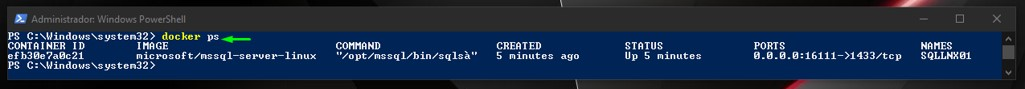
\includegraphics[width=19cm]{./Imagenes/Comando013}
							\end{center}
						\end{figure}
				\subsubsection{Parte 4. Creando un contenedor con Microsoft SQL Server para Windows.}
					\item En el icono deDocker ubicado en el área de notificaciones, hacer click con el botón derecho y utilizar la siguiente opcion.
						\begin{figure}[htb]
							\begin{center}
								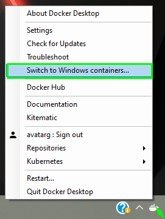
\includegraphics[width=5cm]{./Imagenes/VerIconoDocker}
							\end{center}
						\end{figure}
					\item Ejecutamos el siguiente comando.
						\begin{center}
							\textbf{docker search mssql} \\
						\end{center}
					\item Y el resultado será como se muestra en la siguiente imagen.
						\begin{figure}[htb]						
							\begin{center}
								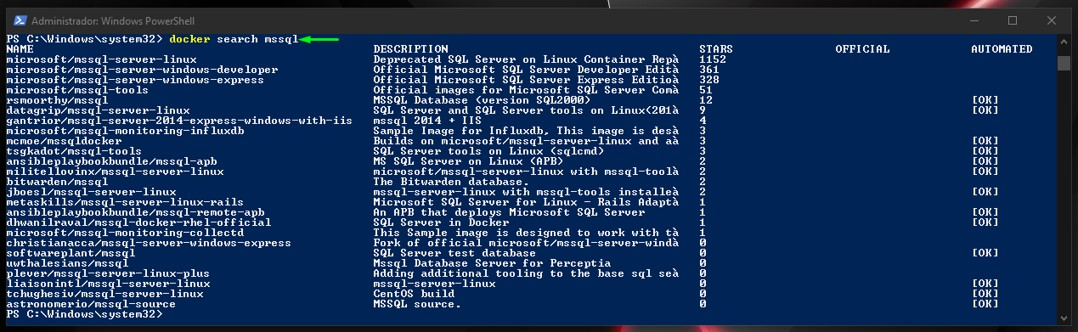
\includegraphics[width=19cm]{./Imagenes/Comando014}
							\end{center}
						\end{figure}
						\vspace{6cm}
					\item Seguimos con la ejecutamos del siguiente comando.
						\begin{center}
							\textbf{docker pull microsoft/mssql-windows-developer} \\
						\end{center}
					\item Lo cual descargará la imagen del contenedor de Microsoft SQL Server en un servidor Linux, como se muestra en la siguiente imagen.
						\begin{figure}[htb]						
							\begin{center}
								\includegraphics[width=19cm]{./Imagenes/Comando015}
							\end{center}
						\end{figure}
					\item Procedemos a ejecutamos el siguiente comando.
						\begin{center}
							\textbf{docker images} \\
						\end{center}
					\item Lo cual deberá visualizar lo siguiente.
						\begin{figure}[htb]						
							\begin{center}
								\includegraphics[width=19cm]{./Imagenes/Comando016}
							\end{center}
						\end{figure}
	\end{itemize}
				\section{Actividades Encargadas.}

	\begin{itemize}
		\subsection{¿Con qué comando(s) exportaría la imagen de Docker de Microsoft SQL Server a otra PC o Servidor?}
			\item Respuesta:
				\begin{figure}[htb]
					\begin{center}
						\includegraphics[width=19cm]{./Imagenes/Comando05}
					\end{center}
				\end{figure}
		\subsection{¿Con qué comando(s) podría generar dos volúmenes para un contenedor para distribuir en un volumen el Archivo de Datos (.mdf) y en otro el Archivo Log (.ldf)?}
			\item Respuesta:
				\begin{figure}[htb]
					\begin{center}
						\includegraphics[width=16cm]{./Imagenes/CrearDataBase}
					\end{center}
				\end{figure}
				\vspace{5cm}
		\subsection{Genere un nuevo contenedor y cree la Base de Datos con las siguientes características.}
			\item Respuesta:
				\begin{figure}[htb]
					\begin{center}
						\includegraphics[width=16cm]{./Imagenes/Generar}
					\end{center}
				\end{figure}
			\item ¿Cuál sería el Script SQL que generaría esta Base de Datos?
	\end{itemize}
				\include{Secciones/Actividad04}
				\include{Secciones/Actividad05}
				\include{Secciones/Actividad06}
\end{document}
